\chapter{DISEÑO DEL PRODUCTO}
\label{cap:diseno}

% La cota de altura es obligatoria: la captura del portal del censador es
% vertical, y a 0.9\textwidth su alto excede la caja de texto.
\newcommand{\capturaui}[4]{%
  \begin{figure}[htbp]
    \centering
    \includegraphics[width=0.9\textwidth,height=0.75\textheight,keepaspectratio]{media/#1}
    \caption[#2]{#3}
    \label{#4}
  \end{figure}%
}

\section{ARQUITECTURA DEL SISTEMA}
\label{sec:arquitectura}
La arquitectura del sistema sigue el patrón de monolito modular: un único servicio
Django \citep{django} con módulos claramente separados por dominio
(\texttt{accounts}, \texttt{datasets}, \texttt{optimization}, \texttt{routes}).

Las tareas de optimización se ejecutan de forma asíncrona mediante Celery
\citep{celery} con Redis como \textit{broker}, dado que el proceso de construcción de
la matriz de costos y la ejecución del \textit{solver} pueden tardar varios minutos
para conjuntos de cien o más puntos.

El motor de ruteo peatonal (OSRM) se despliega localmente en Docker y procesa
datos de \textit{OpenStreetMap} \citep{openstreetmap} de Chile, lo que elimina costos
de API y dependencias de red durante la optimización. La persistencia geográfica se
apoya en la extensión espacial PostGIS de PostgreSQL \citep{postgis}.

La Figura~\ref{fig:arquitectura} resume las capas del sistema y el recorrido de una
optimización: el navegador solicita el trabajo a la API, esta lo encola en Celery en
lugar de resolverlo en el ciclo de la petición HTTP, y el \textit{worker} ejecuta el
\textit{pipeline}, que consulta OSRM para construir la matriz de costos y persiste la
solución en PostGIS. El \textit{frontend} consulta el estado del trabajo por
\textit{polling} hasta que alcanza un estado terminal.

\begin{figure}[H]
  \centering
  % babel-spanish activa '<' y '>'; sin esto, la punta de flecha (>=stealth) no compila
  \shorthandoff{<>}%
  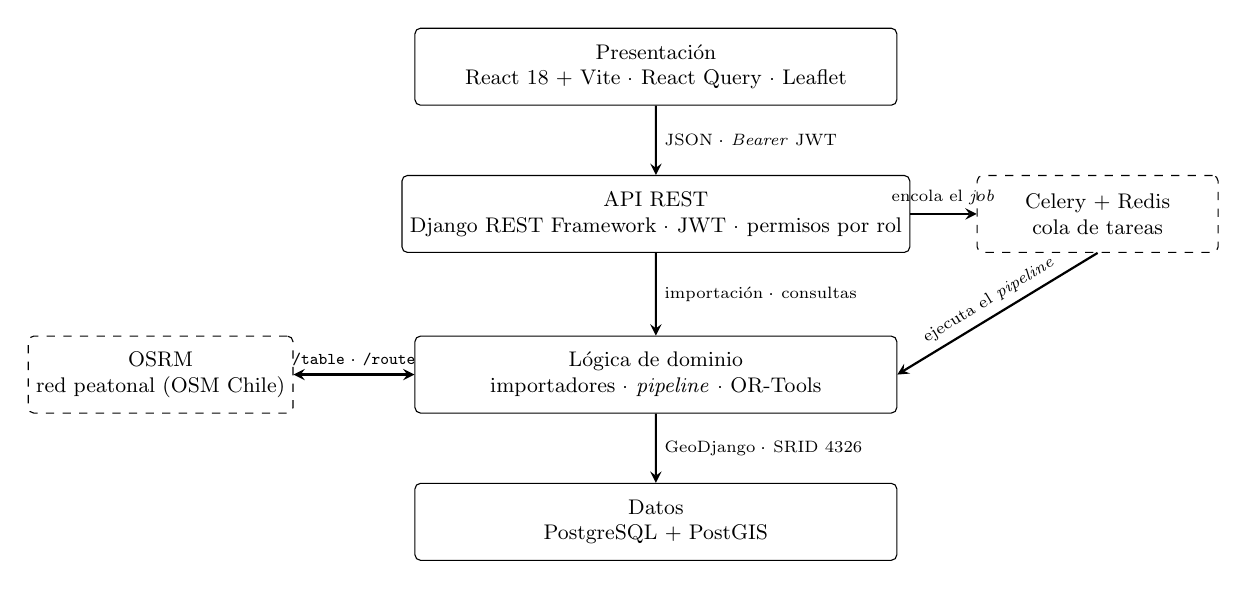
\begin{tikzpicture}[
      scale=0.85, transform shape,
      capa/.style={draw, rounded corners=2pt, align=center, font=\small,
                   minimum width=7.2cm, minimum height=1.15cm},
      externo/.style={draw, dashed, rounded corners=2pt, align=center, font=\small,
                      minimum width=3.6cm, minimum height=1.15cm},
      flujo/.style={->, >=stealth, thick},
      etiqueta/.style={font=\scriptsize, midway}
    ]
    \node[capa]    (p) at (0,0)      {Presentación\\ React 18 + Vite · React Query · Leaflet};
    \node[capa]    (a) at (0,-2.2)   {API REST\\ Django REST Framework · JWT · permisos por rol};
    \node[capa]    (l) at (0,-4.6)   {Lógica de dominio\\ importadores · \textit{pipeline} · OR-Tools};
    \node[capa]    (d) at (0,-6.8)   {Datos\\ PostgreSQL + PostGIS};
    \node[externo] (q) at (6.6,-2.2) {Celery + Redis\\ cola de tareas};
    \node[externo] (o) at (-7.4,-4.6) {OSRM\\ red peatonal (OSM Chile)};

    \draw[flujo] (p) -- (a) node[etiqueta,right] {JSON · \textit{Bearer} JWT};
    \draw[flujo] (a) -- (l) node[etiqueta,right] {importación · consultas};
    \draw[flujo] (l) -- (d) node[etiqueta,right] {GeoDjango · SRID 4326};
    \draw[flujo] (a.east) -- (q.west) node[etiqueta,above] {encola el \textit{job}};
    \draw[flujo] (q.south) -- (l.east) node[etiqueta,above,sloped] {ejecuta el \textit{pipeline}};
    \draw[flujo,<->] (l.west) -- (o.east) node[etiqueta,above] {\texttt{/table} · \texttt{/route}};
  \end{tikzpicture}
  \caption[Arquitectura de Arbocensus]{Arquitectura de Arbocensus. Trazo continuo: capas del monolito Django. Trazo discontinuo: servicios de apoyo desplegados como contenedores independientes.}
  \label{fig:arquitectura}
\end{figure}

% ---- 2.2 -------------------------------------------------------
\section{MODELO DE DATOS}
\label{sec:modelo-datos}

Los modelos de dominio centrales son los siguientes:

\begin{itemize}
  \item \textbf{Dataset}: agrupa un conjunto de árboles importados desde CSV o desde una fuente legada.
  \item \textbf{Tree}: punto geográfico (\texttt{PointField}, SRID 4326) perteneciente a un \texttt{Dataset}. Registra además su procedencia mediante los campos \texttt{source} y \texttt{external\_id}, que identifican la fuente legada y el identificador que el árbol tenía en ella (Sección~\ref{sec:legacy}).
  \item \textbf{RoutingConfig}: parámetros de una sesión de optimización ($T_{\min}$, $T_{\max}$, $s$).
  \item \textbf{OptimizationJob}: tarea de optimización con estado (\texttt{queued}, \texttt{running}, \texttt{completed}, \texttt{failed}) y referencia a la tarea Celery.
  \item \textbf{RoutingSolution}: resultado de un \texttt{OptimizationJob} para una estrategia de partición dada (campo \texttt{strategy}). Almacena el número de rutas $k$, el tiempo total de desplazamiento, el puntaje de balance temporal, las métricas espaciales de la solución (suma de radios máximos, solapamiento total y por ruta, e \textit{IoU} del peor par de rutas) y el desglose de tiempos por fase del \textit{pipeline} (campo \texttt{timing}).
  \item \textbf{Route}: ruta individual con tiempos estimados; su asignación a un censador (\texttt{surveyor}) es opcional.
  \item \textbf{RouteStop}: visita de un árbol en una ruta, con número de secuencia y estado de visita.
  \item \textbf{TreeObservation}: registro histórico del estado de un árbol en un instante dado (Sección~\ref{sec:recenso}). Es la entidad que convierte el sistema en una herramienta de re-censo y no solo de censo inicial.
  \item \textbf{DistanceMatrix}: caché persistente de la matriz $n \times n$ de tiempos OSRM, indexada por un hash SHA-256 de los IDs de árboles activos.
\end{itemize}

La procedencia se modela en el propio \texttt{Tree} en lugar de en una entidad
aparte, porque solo se necesita para dos fines: evitar la doble importación de un
mismo árbol legado y vincular sus observaciones históricas. Una restricción de
unicidad parcial sobre la terna (\texttt{dataset}, \texttt{source},
\texttt{external\_id}), condicionada a \texttt{external\_id} no nulo, impide que un
mismo árbol legado aparezca dos veces en un \textit{dataset} sin restringir a los
árboles importados desde CSV, que no tienen identificador externo.

El orden de visita de cada ruta se deriva de \texttt{RouteStop.sequence};
no existe un campo redundante de secuencia en \texttt{Route}.

Cada \texttt{OptimizationJob} produce una \texttt{RoutingSolution} por cada estrategia
de partición ejecutada (Sección~\ref{sec:estrategias}), lo que permite comparar los
enfoques sobre un mismo conjunto de árboles. Para gobernar cuál de estas soluciones
es la vigente en terreno, el modelo incorpora un ciclo de vida de publicación: el
campo \texttt{published\_at} marca la solución activa de un \textit{dataset} y una
restricción de unicidad parcial (\texttt{UniqueConstraint} condicionada a
\texttt{published\_at} no nulo) garantiza que exista a lo más una
\texttt{RoutingSolution} publicada por \textit{dataset}. Publicar una nueva solución
despublica atómicamente la anterior. La asignación de un censador a una \texttt{Route}
solo se permite sobre la solución publicada, y el campo \texttt{surveyor} admite valor
nulo (\texttt{SET\_NULL}), de modo que las rutas de soluciones no publicadas permanecen
sin asignar hasta que el administrador defina el plan vigente.

La Figura~\ref{fig:er} presenta el modelo entidad-relación simplificado. Se omiten
los atributos no estructurales, así como la relación auxiliar que vincula cada
observación con el usuario que la registra: ese campo es anulable por la misma razón
que lo es el censador de una ruta. Todas las entidades usan claves primarias UUID.

\begin{figure}[H]
  \centering
  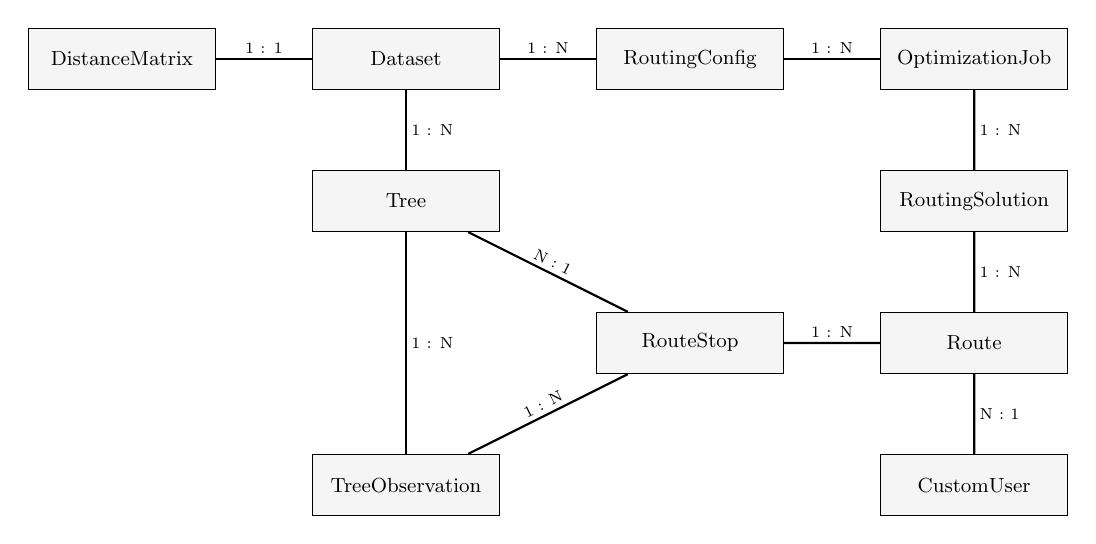
\begin{tikzpicture}[
      scale=0.82, transform shape,
      entidad/.style={draw, fill=black!4, align=center, font=\small,
                      minimum width=2.9cm, minimum height=0.95cm},
      rel/.style={-, thick},
      card/.style={font=\scriptsize, midway, inner sep=2pt}
    ]
    \node[entidad] (dm)  at (-4.4,0)    {DistanceMatrix};
    \node[entidad] (ds)  at (0,0)       {Dataset};
    \node[entidad] (rc)  at (4.4,0)     {RoutingConfig};
    \node[entidad] (job) at (8.8,0)     {OptimizationJob};
    \node[entidad] (tr)  at (0,-2.2)    {Tree};
    \node[entidad] (sol) at (8.8,-2.2)  {RoutingSolution};
    \node[entidad] (rt)  at (8.8,-4.4)  {Route};
    \node[entidad] (rs)  at (4.4,-4.4)  {RouteStop};
    \node[entidad] (obs) at (0,-6.6)    {TreeObservation};
    \node[entidad] (us)  at (8.8,-6.6)  {CustomUser};

    \draw[rel] (ds) -- (dm)  node[card,above] {1 : 1};
    \draw[rel] (ds) -- (rc)  node[card,above] {1 : N};
    \draw[rel] (rc) -- (job) node[card,above] {1 : N};
    \draw[rel] (ds) -- (tr)  node[card,right] {1 : N};
    \draw[rel] (job) -- (sol) node[card,right] {1 : N};
    \draw[rel] (sol) -- (rt) node[card,right] {1 : N};
    \draw[rel] (rt) -- (rs)  node[card,above] {1 : N};
    \draw[rel] (rs) -- (tr)  node[card,above,sloped] {N : 1};
    \draw[rel] (tr) -- (obs) node[card,right] {1 : N};
    \draw[rel] (rs) -- (obs) node[card,above,sloped] {1 : N};
    \draw[rel] (rt) -- (us)  node[card,right] {N : 1};
  \end{tikzpicture}
  \caption[Modelo entidad-relación simplificado]{Modelo entidad-relación simplificado. \texttt{DistanceMatrix} cachea la matriz de tiempos del \textit{dataset}; \texttt{RouteStop} es la fuente de verdad del orden de visita; \texttt{TreeObservation} sobrevive al plan de rutas que la originó.}
  \label{fig:er}
\end{figure}

% ---- 2.3 -------------------------------------------------------
\section{MOTOR DE OPTIMIZACIÓN}

% ---- 2.3.1 ------------------------------------------------------
\subsection{Formulación del Problema}
\label{sec:formulacion}

\subsubsection*{Conjuntos, parámetros y variables}

El problema se define sobre un conjunto de puntos
$P = \{p_1, p_2, \ldots, p_n\}$ correspondientes a las ubicaciones geográficas
de los árboles a censar. Para modelar rutas abiertas ---sin punto de inicio ni de
término predefinido--- se añade un depósito ficticio (\textit{dummy depot})
$p_0$, de modo que el grafo del modelo se define sobre
$V = \{0, 1, \ldots, n\}$, donde el índice $0$ corresponde al depósito y los
índices $1$ a $n$ a los árboles reales. Se dispone de un conjunto
$R = \{1, \ldots, N_{\max}\}$ de vehículos, cuyo cardinal es una cota superior
calculada por la Ecuación~\ref{eq:nmax} y no el número de rutas de la solución.

La función de costo $c_{ij}$ representa el tiempo de caminata entre los
puntos $p_i$ y $p_j$, calculado sobre la red vial peatonal real mediante OSRM. Los
arcos que tocan el depósito tienen costo nulo, $c_{0j} = c_{i0} = 0$, lo que es
precisamente el mecanismo que abre las rutas: entrar y salir del depósito es
gratuito, de modo que la ruta efectiva es la secuencia de árboles que hay entre
ambos extremos. El parámetro $s$ es el tiempo de servicio constante por árbol, y
$d_{ij}$ la distancia de \textit{haversine} entre $p_i$ y $p_j$, empleada por la
dimensión geográfica de la Sección~\ref{sec:estrategias}.

El modelo emplea tres familias de variables de decisión:

\begin{itemize}
  \item $x_{ijr} \in \{0,1\}$: vale $1$ si el vehículo $r$ recorre el arco
        $(i,j)$ y $0$ en caso contrario.
  \item $u_i \in \{0,1\}$, para $i \in \{1,\ldots,n\}$: vale $1$ si el árbol $p_i$
        queda incluido en el plan y $0$ si la solución lo descarta
        (Sección~\ref{sec:disyunciones}).
  \item $z_r \in \{0,1\}$: vale $1$ si el vehículo $r$ queda activo, esto es, si
        se le asigna al menos un árbol.
\end{itemize}

A ellas se añaden las variables acumuladas $t_i \geq 0$ de la dimensión temporal,
que registran el tiempo transcurrido al abandonar el nodo $i$, y su análogo
$g_i \geq 0$ sobre la dimensión geográfica.

\subsubsection*{Restricciones}

Cada árbol incluido en el plan se visita exactamente una vez, y cada visita es
consistente entre la entrada y la salida del nodo:

\begin{equation}
  \sum_{r \in R} \sum_{i \in V} x_{ijr} = u_j, \quad \forall j \in \{1,\ldots,n\}
  \label{eq:grado}
\end{equation}

\begin{equation}
  \sum_{i \in V} x_{ihr} - \sum_{j \in V} x_{hjr} = 0,
  \quad \forall h \in \{1,\ldots,n\},\ \forall r \in R
  \label{eq:flujo}
\end{equation}

La Ecuación~\ref{eq:grado} es la restricción de grado ---un árbol incluido recibe
exactamente un arco entrante, y uno descartado, ninguno--- y la
Ecuación~\ref{eq:flujo} es la conservación de flujo, que impide que un vehículo
entre a un nodo sin salir de él. Cada vehículo activo sale del depósito y regresa a
él a lo sumo una vez:

\begin{equation}
  \sum_{j \in V} x_{0jr} = \sum_{i \in V} x_{i0r} = z_r, \quad \forall r \in R
  \label{eq:deposito}
\end{equation}

La Ecuación~\ref{eq:deposito} liga la activación de un vehículo con su uso efectivo:
un vehículo inactivo no sale del depósito y, por la Ecuación~\ref{eq:flujo}, no puede
tocar nodo alguno. La dimensión temporal, definida en la
Ecuación~\ref{eq:dimension-tiempo}, encadena los tiempos acumulados a lo largo de cada
ruta y acota su valor terminal:

\begin{equation}
  x_{ijr} = 1 \;\Longrightarrow\; t_j \geq t_i + \left\lceil c_{ij} + s\cdot\mathbf{1}[i \neq 0] \right\rceil,
  \qquad t_0 = 0
  \label{eq:dimension-tiempo}
\end{equation}

El tiempo de servicio se carga al abandonar un nodo real y no al llegar a él, y el
depósito ficticio queda exento por la condición $i \neq 0$ del término indicador. El
tiempo total de la ruta del vehículo $r$ es el valor terminal de esa dimensión, que
por la Ecuación~\ref{eq:route_time} equivale al desplazamiento más el servicio de sus
$m_r$ árboles:

\begin{equation}
  T_r = \sum_{(i,j)} c_{ij}\,x_{ijr} + m_r \cdot s
  \label{eq:route_time}
\end{equation}

La única restricción temporal dura del modelo es la cota superior de la
Ecuación~\ref{eq:time_constraints}, implementada como capacidad de la dimensión:

\begin{equation}
  T_r \leq T_{\max}, \quad \forall r \in R
  \label{eq:time_constraints}
\end{equation}

con valores por defecto $T_{\min} = 2\,\text{h}$ y $T_{\max} = 3\,\text{h}$,
parametrizables por el administrador. La cota inferior $T_{\min}$
no es una restricción del modelo sino un objetivo blando: se penaliza el
déficit en la función objetivo en lugar de prohibirlo, por la razón que se detalla
en la Sección~\ref{sec:solver}. En consecuencia, una solución puede presentar rutas
de duración inferior a $T_{\min}$, y de hecho las presenta: la solución de
producción reportada en el Capítulo~\ref{cap:resultados} tiene tres.

\subsubsection*{Función objetivo}

El modelo es monobjetivo: los tres propósitos enunciados más abajo se escalarizan
en una suma ponderada de seis términos, y no se resuelven de forma lexicográfica ni
se construye un frente de Pareto. La función que el \textit{solver} minimiza es

\begin{equation}
  \begin{aligned}
    \min \quad
      &\underbrace{\sum_{r \in R} \sum_{(i,j)} \left\lceil c_{ij} + s\cdot\mathbf{1}[i \neq 0] \right\rceil x_{ijr}}_{\text{costo de arco}}
      \;+\; \underbrace{C_{\text{fijo}} \sum_{r \in R} z_r}_{\text{flota}} \\[2pt]
      &+\; \underbrace{\alpha \sum_{r \in R} \max\!\left(0,\; T_{\min} - T_r\right)}_{\text{penalización inferior}}
      \;+\; \underbrace{\beta \sum_{r \in R} \max\!\left(0,\; T_r - \tau\right)}_{\text{penalización superior}} \\[2pt]
      &+\; \underbrace{\pi \sum_{i=1}^{n} \left(1 - u_i\right)}_{\text{descarte}}
      \;+\; \underbrace{\lambda_{\text{span}} \sum_{r \in R} \operatorname{span}_r}_{\text{extensión geográfica}}
  \end{aligned}
  \label{eq:objetivo}
\end{equation}

donde $\operatorname{span}_r = \max_i g_i - \min_i g_i$ sobre los nodos del
vehículo $r$ es la extensión de la ruta en la dimensión geográfica, y las
constantes toman los valores de la Tabla~\ref{tab:coeficientes}. Las penalizaciones
inferior y superior se aplican, en la implementación, sobre la variable acumulada
del nodo terminal de cada vehículo, que es donde $t_i$ vale $T_r$; un vehículo
inactivo no contribuye a ninguno de los seis términos.

\begin{table}[H]
  \centering
  \caption{Coeficientes de la función objetivo y su magnitud en la configuración de producción.}
  \label{tab:coeficientes}
  \small
  \begin{tabularx}{\textwidth}{@{}l l l X@{}}
    \toprule
    Símbolo & Término & Valor & Unidad y lectura \\
    \midrule
    --- & Costo de arco & $1$ & Por segundo de tránsito: el término que expresa el tiempo de caminata que el modelo minimiza. \\
    $C_{\text{fijo}}$ & Costo fijo de vehículo & $100\,000$ & Por vehículo activo. Es el mecanismo que minimiza la flota (Sección~\ref{sec:flota}). \\
    $\alpha$ & Penalización inferior & $10\,000$ & Por segundo en que $T_r$ queda bajo $T_{\min}$. \\
    $\beta$ & Penalización superior & $500$ & Por segundo en que $T_r$ supera el objetivo blando $\tau$. \\
    $\tau$ & Objetivo blando superior & $(T_{\min}+T_{\max})/2$ & En segundos: el punto medio del intervalo de jornada. \\
    $\pi$ & Penalización de descarte & $10^{6}$ & Por árbol excluido del plan, esto es $10\,C_{\text{fijo}}$ (Sección~\ref{sec:disyunciones}). \\
    $\lambda_{\text{span}}$ & Coeficiente de extensión geográfica & $3$ & Por metro de extensión de la ruta en la dimensión de \textit{haversine} (Sección~\ref{sec:estrategias}). \\
    \bottomrule
  \end{tabularx}
\end{table}

Los tres propósitos que la Ecuación~\ref{eq:objetivo} escalariza son:

\begin{enumerate}
  \item Minimizar el número de rutas $k = \sum_r z_r$, a través del término de flota.
  \item Minimizar el tiempo total de desplazamiento, a través del costo de arco.
  \item Reducir el desbalance de carga entre rutas, a través de las dos penalizaciones
        blandas que empujan cada $T_r$ hacia el intervalo $[T_{\min},\,\tau]$.
\end{enumerate}

Corresponde precisar el tercero, porque su enunciado usual ---«minimizar la
desviación estándar de $T_r$»--- no describe lo que el modelo hace. Una desviación
estándar es una propiedad del conjunto de rutas y no se puede expresar como costo
aditivo por arco, que es la única forma que admite la formulación: el
\textit{solver} evalúa un costo por cada arco recorrido y por cada variable
acumulada terminal, nunca un estadístico de la solución completa. Lo que el modelo
implementa son las dos penalizaciones blandas bilaterales de la
Ecuación~\ref{eq:objetivo}, y lo que el Capítulo~\ref{cap:resultados} reporta como
balance es un tercer objeto, el cociente $\min_r T_r / \max_r T_r$. Los tres
---objetivo declarado, mecanismo implementado y métrica reportada--- apuntan en la
misma dirección, pero no son la misma cantidad, y en esta memoria se nombran por
separado.

Conviene situar el modelo dentro de la taxonomía de la investigación operativa
\citep{toth2014vehicle}, porque la denominación abreviada \textit{Open mTSP} omite
tres extensiones que sí están presentes y que determinan la solución. Las rutas
abiertas ---sin depósito de partida ni de retorno--- corresponden al \textit{Open
Vehicle Routing Problem} \citep{li2007open}, y aquí se obtienen mediante el depósito
ficticio de costo nulo descrito más arriba. Las visitas opcionales penalizadas sitúan
el modelo en la familia de los problemas de ruteo con beneficios o
\textit{prize-collecting} \citep{balas1989prize,feillet2005traveling}, en los que
omitir un nodo no es infactible sino costoso. Y la dimensión acumulativa con capacidad
dura $T_{\max}$ es estructuralmente una restricción de capacidad, aunque su unidad sea
el tiempo y no la carga. El caso base sin ninguna de las tres es el \textit{Multiple
Travelling Salesman Problem} \citep{bektas2006multiple,laporte1992traveling}, y la
combinación de varias de ellas sobre un mismo modelo es lo que la literatura reciente
denomina un problema de ruteo multiatributo \citep{vidal2013heuristics}.

La escala relativa de los coeficientes importa más que sus valores absolutos, y
conviene leerla en términos marginales, esto es, como el precio de un segundo
adicional de caminata en una ruta. Con los valores por defecto, ese precio es de
$-9\,999$ mientras la ruta está por debajo de $T_{\min}$ ---el \textit{solver} está
pagado por alargarla---, de $+1$ entre $T_{\min}$ y el objetivo blando $\tau$, y de
$+501$ por encima de $\tau$. Esa asimetría, y no el costo de arco, es el canal
dominante del objetivo, y explica los resultados de sensibilidad a las
penalizaciones de la Sección~\ref{sec:discusion-calidad}.

% ---- 2.3.2 ------------------------------------------------------
\subsection{Construcción de la Matriz de Costos}
\label{sec:matriz}

La matriz de costos $C \in \mathbb{R}^{n \times n}$ se construye consultando el
\textit{endpoint} \texttt{/table/v1/foot} de OSRM \citep{osrm}, que devuelve los
tiempos de caminata reales entre todos los pares de puntos en una única solicitud
HTTP. El servicio resuelve esas consultas sobre el grafo de \textit{OpenStreetMap}
preprocesado con el algoritmo \textit{Multi-Level Dijkstra}, que particiona la red en
niveles jerárquicos y precalcula atajos entre celdas, lo que permite responder
consultas de camino mínimo en tiempo prácticamente independiente de la longitud del
trayecto \citep{delling2017customizable}.

Para evitar recomputaciones costosas, la matriz se persiste en el modelo
\texttt{DistanceMatrix} asociado al \textit{dataset}.
La clave de caché es un hash SHA-256 calculado sobre los identificadores de los
árboles activos ordenados; si el conjunto de árboles cambia, el hash no coincide
y la matriz se recalcula automáticamente.

Los nodos inalcanzables (devueltos como \texttt{null} por OSRM) se reemplazan por
una penalización de $9\,999\,999$ segundos, lo que garantiza la viabilidad numérica
del \textit{solver}: la matriz queda sin valores nulos y toda operación aritmética
sobre ella está definida. La sustitución sí altera la topología de la solución, y esa
es justamente su función: un arco de ese costo excede cualquier cota de jornada
concebible, de modo que ninguna ruta puede incorporarlo y el nodo afectado termina
descartado por la disyunción que lo cubre (Sección~\ref{sec:disyunciones}). Lo que la
penalización evita no es el cambio de topología sino la propagación de valores nulos
al modelo.

El factor que limita el tamaño de una consulta no es el parámetro
\texttt{--max-table-size} de OSRM (fijado en $5\,000$), sino la longitud máxima de
la URL: el servicio \texttt{/table} codifica cada coordenada en la propia ruta de la
petición, de modo que la solicitud falla por longitud de URL antes de alcanzar el
límite de tabla. El sistema fija por ello un tope de $350$ árboles por solicitud.
Cuando el \textit{dataset} lo supera, la matriz se construye por fragmentación
(\textit{chunking}): los puntos se dividen en bloques de $175$ coordenadas
---la mitad del tope, ya que cada petición fragmentada transporta simultáneamente
las coordenadas del bloque origen y las del bloque destino--- y se solicita un
bloque $(i,j)$ de la matriz por cada par de bloques, empleando los parámetros
\texttt{sources} y \texttt{destinations} de OSRM. El número de solicitudes crece
así de forma cuadrática con el número de bloques, lo que domina el costo de la
primera construcción de la matriz para \textit{datasets} grandes
(Capítulo~\ref{cap:resultados}). Un tope adicional de $2\,000$ árboles acota la
dimensión de la matriz, cuyo tamaño en disco crece como $O(n^2)$.

% ---- 2.3.3 ------------------------------------------------------
\subsection{Estimación del Número de Rutas}

\label{sec:flota}

El número de rutas $k$ ---y por lo tanto el número de censadores que deben salir a
terreno en una jornada--- no es un dato de entrada del sistema: es una salida del
\textit{solver}. El administrador nunca declara cuántos equipos tiene disponibles; declara
cuánto puede durar una jornada ($T_{\min}$, $T_{\max}$) y cuánto toma censar un
árbol ($s$), y el sistema deriva la flota necesaria. Esta decisión de diseño evita
el enfoque de iteración externa ---resolver el modelo con $1, 2, 3, \ldots$
vehículos hasta hallar el menor valor factible---, que multiplica el tiempo de
cómputo por el número de intentos y resulta frágil, pues una corrida infactible no
distingue entre «faltan vehículos» y «el modelo no admite solución».

En su lugar, el sistema entrega a \textit{OR-Tools} un techo $N_{\max}$ de vehículos
disponibles y deja que el \textit{solver} decida cuántos activa. El techo se calcula a partir
del trabajo total estimado ---servicio más desplazamiento--- dividido por la duración
mínima de una ruta:

\begin{equation}
  N_{\max} = \min\!\left(n,\;
  \left\lceil \frac{n \cdot s + n \cdot \hat{c}_{\text{nn}}}{T_{\min}} \right\rceil + b
  \right)
  \label{eq:nmax}
\end{equation}

donde $n$ es el número de árboles activos, $s$ el tiempo de servicio por árbol y
$\hat{c}_{\text{nn}}$ el tiempo medio al vecino más cercano: el promedio,
sobre todos los nodos, del arco de menor costo que sale de cada nodo, excluyendo la
diagonal y los pares inalcanzables (aquellos con la penalización de $9\,999\,999$\,s).
Se emplea el vecino más cercano y no el promedio de todos los pares porque una ruta
real encadena árboles contiguos, no pares arbitrarios: el promedio general
sobreestima el desplazamiento por árbol en un factor que crece con la extensión
geográfica del \textit{dataset}, e inflaría $N_{\max}$ innecesariamente. El término
$b$ es un margen de holgura de $5$ vehículos, y el mínimo con $n$ impide que el techo
supere el caso degenerado de un árbol por ruta.

Es importante subrayar que $N_{\max}$ es una cota superior, no una
predicción: solo debe ser lo bastante amplia como para no excluir la solución óptima.
La minimización efectiva de $k$ ocurre dentro del \textit{solver}, mediante el costo fijo de
$100\,000$\,s por vehículo activo (Sección~\ref{sec:solver}): activar una ruta
adicional es tan caro que el \textit{solver} solo lo hace cuando las restricciones temporales
lo obligan. El número de rutas de la solución final es, en la práctica,
sustancialmente menor que $N_{\max}$.

La misma estimación alimenta un segundo uso, orientado a la planificación operativa
y no al \textit{solver}: el \textit{endpoint} \texttt{GET /api/optimization/estimate/} permite
al administrador consultar, antes de lanzar una optimización, cuántos censadores
requeriría un \textit{dataset} bajo un $T_{\min}$ y un tiempo de servicio dados. En
este caso la Ecuación~\ref{eq:nmax} se evalúa con margen nulo ($b=0$), pues aquí sí
interesa una estimación ajustada y no un techo. La consulta reutiliza la matriz de
costos en caché y no dispara ninguna consulta a OSRM: si el \textit{dataset} aún no
tiene matriz calculada, el sistema responde que la estimación no está disponible en
lugar de incurrir en el costo de construirla.

% ---- 2.3.4 ------------------------------------------------------
\subsection{Solver VRP con OR-Tools}
\label{sec:solver}

La formulación en \textit{OR-Tools} usa el modelo de ruteo vehicular (\textit{Vehicle Routing
Problem}) con las siguientes características:

\begin{itemize}
  \item \textbf{Rutas abiertas}: se introduce un depósito ficticio (\textit{dummy depot})
        en el nodo 0 con costo de tránsito cero hacia todos los nodos reales.
        Los nodos reales se indexan de $1$ a $n$.
  \item \textbf{Cota superior de tiempo ($T_{\max}$, restricción dura)}:
        implementada mediante \texttt{AddDimension} con capacidad máxima $T_{\max}$.
        Ninguna ruta puede superar este valor.
  \item \textbf{Cota inferior de tiempo ($T_{\min}$, restricción blanda)}:
        implementada mediante \texttt{SetCumulVarSoftLowerBound} en el nodo terminal
        de cada vehículo, con coeficiente de penalización $10\,000$.
        Una cota inferior dura volvería el modelo infactible cuando el número de rutas
        necesarias multiplicado por $T_{\min}$ supera el trabajo disponible; la
        formulación blanda evita esa infactibilidad al penalizar el déficit en lugar de
        prohibirlo.
  \item \textbf{Balance de rutas}:
        \texttt{SetCumulVarSoftUpperBound} dirige las rutas hacia el punto medio
        $(T_{\min} + T_{\max})/2$, lo que reduce la varianza entre rutas.
  \item \textbf{Minimización de rutas activas}:
        costo fijo de $100\,000$ por vehículo descarta vehículos innecesarios.
  \item \textbf{Disyunciones por nodo}:
        cada árbol puede quedar fuera de la solución a un costo de
        $1\,000\,000$ (Sección~\ref{sec:disyunciones}).
  \item \textbf{Búsqueda local}:
        estrategia \textit{Guided Local Search} (GLS)
        \citep{voudouris1999guided} con solución inicial
        \textit{PATH\_CHEAPEST\_ARC} ---una construcción voraz por arco más barato,
        de la misma familia que el clásico algoritmo de ahorros
        \citep{clarke1964scheduling}---, con tiempo límite configurable. A falta de
        un valor explícito, el \textit{pipeline} lo deriva del tamaño del problema
        como $\min(30 + 1{,}5\,n,\ 120)$ segundos, de modo que un \textit{dataset}
        pequeño no consume el presupuesto completo; para los tamaños de esta
        memoria la expresión satura en su tope de $120$\,s.
\end{itemize}

Si el \textit{solver} no encuentra solución, el \textit{pipeline} no falla en silencio: emite
un error que reporta el número de árboles y los parámetros de configuración vigentes
(tiempo de servicio y $T_{\max}$), de modo que el administrador pueda identificar qué
restricción relajar.

% ---- 2.3.5 ------------------------------------------------------
\subsection{Disyunciones de nodos}
\label{sec:disyunciones}

Un modelo VRP en el que todos los nodos son obligatorios es un modelo que puede
resultar infactible. Basta un único árbol cuyo tiempo de acceso ---ida y
vuelta desde cualquier otro nodo, más su tiempo de servicio--- exceda la cota dura
$T_{\max}$ para que no exista ninguna asignación válida y el \textit{solver} retorne sin
solución. En el contexto de este problema esa situación es realista: los
\textit{datasets} provienen de censos reales y contienen árboles geográficamente
aislados, así como nodos que OSRM no logra enrutar sobre la red peatonal y que, en
consecuencia, reciben la penalización de $9\,999\,999$\,s en la matriz de costos
(Sección~\ref{sec:matriz}). Sin un mecanismo de escape, un solo árbol de este tipo invalidaría
la planificación de todo el \textit{dataset}, que es precisamente el modo de falla
que el sistema debe evitar.

La solución adoptada consiste en declarar cada nodo real como una
\textit{disyunción} unitaria mediante \texttt{AddDisjunction}, asignándole una
penalización $\pi$ por omisión. Formalmente, el modelo deja de exigir que todo árbol
sea visitado y pasa a minimizar el costo de las rutas más $\pi$ por cada árbol
descartado. La factibilidad queda así garantizada por construcción: siempre existe
al menos una solución ---aquella que descarta los nodos problemáticos--- y el \textit{solver}
nunca queda sin respuesta por culpa de un puñado de árboles inalcanzables.

La calibración de $\pi$ es la decisión de diseño relevante. El sistema fija

\begin{equation}
  \pi = 10 \cdot C_{\text{fijo}} = 10 \cdot 100\,000 = 1\,000\,000
  \label{eq:drop_penalty}
\end{equation}

La Ecuación~\ref{eq:drop_penalty} sitúa la penalización un orden de magnitud por
sobre el costo fijo de activar un vehículo. La
relación entre ambas constantes ---y no sus valores absolutos--- es lo que gobierna
el comportamiento del \textit{solver}: descartar un árbol es diez veces más caro que abrir una
ruta entera para él. En consecuencia, mientras exista alguna ruta factible que pueda
absorber al árbol, el \textit{solver} siempre preferirá crearla antes que omitirlo, y el
descarte queda reservado a los nodos que ninguna ruta puede alojar sin violar la cota
dura $T_{\max}$. La disyunción actúa entonces como válvula de seguridad, no como
mecanismo de optimización: no se usa para «podar» árboles caros, sino para no perder
la solución completa por culpa de los imposibles.

Los árboles descartados no se pierden ni se ocultan: el \textit{pipeline} los extrae
de la solución ---son los nodos cuya variable de sucesión apunta a sí misma--- y los
propaga como parte del resultado del trabajo de optimización (campo
\texttt{dropped\_trees}), de modo que el administrador sabe exactamente qué árboles
quedaron fuera del plan y puede tratarlos como excepciones. El comportamiento
observado en el \textit{dataset} real es consistente con la calibración descrita: en
la grilla de seis variantes operacionales de la Tabla~\ref{tab:grilla-spatial}, solo
las dos variantes de $T_{\max}=2$\,h con tiempo de servicio alto descartan árboles
---un árbol con servicio de $2$\,min y dos con servicio de $3$\,min---, de forma
consistente en las tres semillas; las cuatro variantes restantes alcanzan cobertura
total.

El costo de esta garantía es de espacio de búsqueda: cada nodo incorpora una
decisión binaria adicional ---visitarlo u omitirlo---, lo que amplía el vecindario
que la metaheurística debe explorar en cada iteración. Dado que la búsqueda local
está acotada por un límite de tiempo de reloj y que el GLS concentra prácticamente
todo el tiempo de ejecución del \textit{pipeline}
(Capítulo~\ref{cap:resultados}), cabe esperar que el efecto no se manifieste como un
mayor tiempo total sino como una menor calidad alcanzable dentro del mismo
presupuesto. Esa expectativa no se verificó experimentalmente y se asume como
limitación del trabajo (Sección~\ref{sec:posibles-mejoras}).

% ---- 2.3.6 ------------------------------------------------------
\subsection{Estrategias de partición espacial}
\label{sec:estrategias}

La formulación global anterior minimiza el tiempo total de recorrido y equilibra
la duración de las rutas, pero no incorpora ningún criterio geográfico explícito
en la partición de los nodos. Como consecuencia, las rutas se agrupan por
proximidad temporal y no espacial, lo que produce \textit{solapamiento}
(\textit{interleaving}) entre rutas distintas que crece con la densidad de árboles
(véase la Sección de resultados). El sistema implementa por ello tres estrategias de
partición, seleccionables al crear el trabajo de optimización mediante el campo
\texttt{strategy}. Un cuarto valor, \texttt{compare}, ejecuta las tres sobre el mismo
conjunto de árboles y persiste una \texttt{RoutingSolution} independiente por
estrategia, lo que permite contrastarlas bajo una misma matriz de costos y un mismo
presupuesto de \textit{solver}; es el modo con que se produjeron las comparaciones del
Capítulo~\ref{cap:resultados}. La estrategia \texttt{global} reproduce el
comportamiento de la formulación anterior sin cambios y constituye la línea base;
la estrategia seleccionada por defecto es \texttt{spatial\_term}, a la luz de los
resultados de la comparación (Capítulo~\ref{cap:resultados}).

\begin{itemize}
  \item \textbf{\texttt{global}}: el \textit{Open mTSP} único descrito en la
        Sección~\ref{sec:solver}, sin término espacial. Constituye la línea base.
  \item \textbf{\texttt{spatial\_term}}: añade una segunda dimensión de
        \textit{distancia geográfica} ---la fórmula de \textit{haversine} entre
        paradas \citep{sinnott1984virtues}--- y penaliza la
        extensión geográfica de cada ruta mediante
        \texttt{SetSpanCostCoefficientForAllVehicles} con coeficiente
        $\lambda_{\text{span}} = 3$. El \textit{span} de una ruta es la diferencia
        entre el máximo y el mínimo acumulado de la dimensión a lo largo del
        vehículo; penalizarlo empuja al \textit{solver} hacia rutas más compactas a costa
        de mayor tiempo total. La cota superior temporal se ajusta al punto medio
        $(T_{\min} + T_{\max})/2$ para preservar el balance.
  \item \textbf{\texttt{cluster\_first}}: enfoque \textit{cluster-first,
        route-second}, esto es, resolver primero la asignación de nodos a grupos y
        después un recorrido por grupo \citep{fisher1981generalized}. Primero se
        proyectan las coordenadas a un plano local mediante una aproximación
        equirectangular y se particionan en $k$ grupos con el algoritmo de Lloyd
        \citep{lloyd1982least} bajo la inicialización \textit{k-means++}
        \citep{arthur2007kmeans}, que elige los centros iniciales con probabilidad
        proporcional al cuadrado de su distancia al centro más cercano ya escogido y
        acota en esperanza el error respecto del óptimo; el número de grupos $k$ se
        estima a partir de la
        carga de trabajo por árbol (servicio más desplazamiento promedio) sobre el
        tiempo objetivo. Luego se resuelve un VRP independiente por grupo con el
        mismo \texttt{ArbocensusVRPSolver}, lo que acota la dispersión geográfica
        de cada ruta por construcción. Una aserción de cobertura verifica que la
        unión de los grupos cubra exactamente el conjunto de árboles.
\end{itemize}

% ---- 2.3.7 ------------------------------------------------------
\subsection{Post-proceso de resecuenciación intra-ruta}
\label{sec:postpass}

La asignación de árboles a rutas y el orden de visita dentro de cada ruta son dos
decisiones que el \textit{solver} toma de forma simultánea, bajo un presupuesto de
tiempo que se agota antes de que la búsqueda converja
(Capítulo~\ref{cap:resultados}). Al cortarse por reloj de pared, el GLS entrega
soluciones en las que la asignación ya es buena pero el ordenamiento interno de
alguna ruta conserva cruces que un refinamiento local elimina de inmediato. El
sistema explota esa asimetría con un post-proceso que se aplica a toda solución
antes de persistirla, sin condición ni parámetro que lo desactive.

El procedimiento es un 2-opt de camino abierto \citep{croes1958method,lin1965computer},
aplicado a cada ruta de forma independiente. Dada la secuencia de paradas de una
ruta, examina todo par de posiciones no adyacentes, invierte el segmento comprendido
entre ellas y conserva la inversión cuando reduce el costo del camino; repite el
barrido hasta que ninguna inversión mejora. La variante es de camino \textit{abierto}
---y no la clásica de circuito--- porque las rutas del problema no se cierran sobre
un depósito: al invertir un segmento que llega hasta el último nodo, el costo del
arco de retorno no existe y no debe contabilizarse.

Tres propiedades hacen que el post-proceso sea seguro incorporarlo de forma
incondicional:

\begin{itemize}
  \item \textbf{Optimiza la misma magnitud que el \textit{solver}.} El 2-opt evalúa
        las inversiones sobre la matriz de tiempos de OSRM, exactamente la misma que
        alimenta el costo de arco de la Ecuación~\ref{eq:objetivo}. No introduce un
        criterio nuevo ni una geometría distinta.
  \item \textbf{Nunca empeora una ruta.} Solo acepta una inversión cuando el costo
        del camino disminuye, de modo que el tiempo de desplazamiento de cada ruta
        es menor o igual al que entregó el \textit{solver}, y el de la solución
        completa también.
  \item \textbf{No altera nada más.} Reordena las paradas dentro de cada ruta, sin
        mover un árbol de una ruta a otra. La asignación, el número de rutas $k$, el
        conjunto de árboles descartados y el número de paradas por ruta quedan
        intactos. El índice de balance, en cambio, no queda garantizado: como es el
        cociente $\min_r T_r / \max_r T_r$, puede subir o bajar según cuál sea la
        ruta que el refinamiento acorta, aunque ninguna duración aumente.
\end{itemize}

Su costo computacional es despreciable frente al del \textit{solver}. Cada barrido
examina $O(m_r^2)$ pares para una ruta de $m_r$ paradas y el procedimiento repite
barridos hasta el óptimo local; como la carga de servicio acota $m_r$ a unas
decenas de árboles en las configuraciones operacionales, el post-proceso completo se
ejecuta en un tiempo que no aparece en el desglose por fases del
\textit{pipeline}, dominado por los $120$\,s del GLS
(Sección~\ref{sec:perfil-rendimiento}).

La adopción de este post-proceso como comportamiento por defecto no fue inmediata:
una primera evaluación lo rechazó por empeorar la métrica de auto-cruces, y solo la
corrección posterior de esa métrica ---que medía sobre cuerdas rectas y no sobre el
trazado real de calles--- permitió establecer que el algoritmo mejora
simultáneamente el tiempo de viaje y la geometría real. Esa historia, y la medición
que la cierra, se documentan en la Sección~\ref{sec:discusion-calidad}.

% ---- 2.4 -------------------------------------------------------
\section{IMPORTACIÓN Y SELECCIÓN DE FUENTES LEGADAS}
\label{sec:legacy}

El sistema no parte de cero: existen dos bases de datos operativas de versiones
anteriores del proyecto Arbocensus
\citep{binder-cortes2023,pizarro-zumaeta2024}, que contienen el arbolado ya catastrado
en campañas previas. Ambas se incorporan como fuentes de importación, identificadas por
el campo \texttt{source} del modelo \texttt{Tree}:

% Orden cronológico confirmado por los volcados de las bases (migraciones y muestras):
% legacy_app (esquema arbocensus_app_*, muestras por QR) es la más antigua: génesis de
% base 2021-10 y capturas de terreno desde 2021-10; mapea a la app de censado inicial
% (repo mrecabarren/arbocensus). legacy_api (arbocensus_api_app_*, posición/especie
% explícitas, real_tree_id) es posterior: génesis 2023-06 y capturas desde 2023-06; NO
% corresponde a la ludificación 2023 (fastAPI, modelos badge/score/campaign, sin datos de
% identificación de árboles). La asignación de cada base a una MEMORIA concreta sigue
% siendo inferencia por esquema (no consta en las fuentes), por lo que el texto cita ambas
% memorias en conjunto; pero el orden relativo app-antes-que-api sí está respaldado por
% los timestamps de los volcados. Por eso se presenta primero legacy_app.
\begin{itemize}
  \item \texttt{legacy\_app} (esquema \texttt{arbocensus\_app\_*}): la más antigua, base
        de la aplicación de censado previa ---una aplicación web orientada a dispositivos
        móviles---, donde el árbol no tiene una posición canónica sino
        un conjunto de muestras (\textit{samples}) tomadas en terreno, cada una con
        su propia lectura de GPS. La posición de cada árbol se reconstruye como la
        mediana de las latitudes y longitudes de sus muestras, agrupadas por
        código QR, descartando las lecturas sin coordenada y aquellas con latitud
        igual a cero ---el valor con que la aplicación previa dejaba constancia de una
        lectura de GPS fallida---. Se emplea la
        mediana y no el promedio por su robustez frente a lecturas de GPS
        atípicas, habituales en captura urbana bajo copa arbórea. De este modo se
        obtienen $1\,178$ árboles con posición utilizable.
  \item \texttt{legacy\_api} (esquema \texttt{arbocensus\_api\_app\_*}): posterior a la
        anterior, aporta $429$ árboles con posición explícita y especie, organizados en
        áreas pertenecientes a campañas de censo.
\end{itemize}

El \textit{dataset} definitivo de la evaluación reúne ambas fuentes y totaliza
$n = 1\,607$ árboles. El acceso a las bases legadas es estrictamente de solo
lectura (la conexión se abre con \texttt{readonly}), dado que se trata de sistemas
que no pertenecen al alcance de esta iteración del proyecto y cuya integridad no debe verse
comprometida por el proceso de importación.

\subsection{Selección previa a la creación del dataset}

La decisión de diseño central de este módulo es que \textbf{la importación no crea
un \textit{dataset} de forma inmediata}. Importar áreas completas a ciegas ---el
enfoque inicial--- resultaba inadecuado en la práctica: el usuario no sabe, antes de
importar, qué árboles trae un área, cuáles ya están en el sistema ni si el conjunto
resultante corresponde al territorio que efectivamente quiere censar. El flujo se
divide por ello en dos etapas: primero \textbf{explorar y seleccionar}, y solo
después \textbf{materializar} el \textit{dataset} con la selección confirmada.

La exploración se sirve de dos \textit{endpoints} de solo lectura que no escriben
nada en la base de datos. El primero,
\texttt{GET /api/datasets/legacy/areas/}, lista las áreas de censo con su campaña, su
número de árboles y su polígono; como la fuente \texttt{legacy\_api} almacena las
áreas como listas de vértices y no como geometrías, el polígono se reconstruye
---cerrando el anillo si la fuente no lo entrega cerrado--- y la pertenencia de cada
árbol a un área se determina por inclusión punto-en-polígono, no por una clave
foránea, que la fuente no provee. El segundo,
\texttt{GET /api/datasets/legacy/trees/}, devuelve el arbolado de ambas fuentes con
su posición, su especie, el área que lo contiene y una marca
\texttt{already\_imported} que indica si ese árbol ya fue traído a un \textit{dataset}
del sistema. Si la variable de entorno de una fuente no está configurada, el sistema
responde con un código 503 explícito en lugar de degradarse silenciosamente.

\begin{sloppypar}
La materialización ocurre en un único paso transaccional mediante
\texttt{POST /api/datasets/from-legacy-selection/}, que recibe el nombre del
\textit{dataset} y la lista de árboles seleccionados. Cabe notar que el contrato
identifica cada árbol por el par (\texttt{source}, \texttt{external\_id}) y no por un
identificador plano: al coexistir dos fuentes con espacios de identificadores
independientes, un \texttt{external\_id} por sí solo es ambiguo. El
\textit{endpoint} crea el \texttt{Dataset}, sus \texttt{Tree} y el histórico de
observaciones asociado (Sección~\ref{sec:recenso}) dentro de una misma transacción,
de modo que un fallo parcial no deja \textit{datasets} a medio poblar.
\end{sloppypar}

Existe además un \textit{endpoint} auxiliar,
\texttt{POST /api/datasets/import-legacy/}, que importa un área completa o la
totalidad de la fuente sin selección previa. No forma parte del flujo del usuario y
no tiene interfaz asociada: se conserva como atajo programático para construir
\textit{datasets} de forma reproducible en los experimentos del
Capítulo~\ref{cap:resultados}.

\subsection{Mapa de selección}

La interfaz de selección (\texttt{LegacyImport}, con el componente
\texttt{LegacySelectionMap}) presenta sobre un mapa \textit{Leaflet} la totalidad del arbolado
legado y los polígonos de las áreas de censo. Cada árbol se dibuja como un marcador
circular cuyo color codifica su estado: disponible, seleccionado o ya importado ---
estos últimos, además, no son interactivos, lo que hace imposible seleccionar dos
veces el mismo árbol---. La selección puede componerse mediante tres mecanismos
combinables:

\begin{enumerate}
  \item \textbf{Por área}: al hacer clic sobre el polígono de un área se alternan de
        una vez todos los árboles contenidos en ella.
  \item \textbf{Por rectángulo} (\textit{bounding box}): un modo de arrastre permite
        trazar un rectángulo sobre el mapa y agregar a la selección todos los árboles
        comprendidos en sus límites, con independencia del área a la que pertenezcan.
  \item \textbf{Por árbol individual}: el clic sobre un marcador agrega o quita ese
        árbol de la selección.
\end{enumerate}

Un panel lateral mantiene visible la selección acumulada y permite la
\textbf{des-selección manual} de cualquier árbol, de forma que los tres mecanismos
anteriores actúan como brochas gruesas que el usuario refina antes de confirmar. Solo
al confirmar ---indicando el nombre del \textit{dataset}--- se emite la solicitud de
creación. El resultado es que el recorte territorial del censo es una decisión
explícita del administrador, tomada sobre la evidencia cartográfica, y no una
consecuencia de cómo estaban organizadas las áreas en el sistema anterior.

\capturaui{ui-legacy-import.png}{Mapa de selección de arbolado legado}{Mapa de selección de arbolado legado (\texttt{/admin/datasets/legacy-import}): polígonos de las áreas de censo, marcadores coloreados por estado (disponible, seleccionado, ya importado) y panel lateral de la selección acumulada.}{fig:ui_legacy}

% ---- 2.5 -------------------------------------------------------
\section{RE-CENSO Y REGISTRO DE OBSERVACIONES}
\label{sec:recenso}

Un censo de arbolado urbano no es un evento único sino un proceso recurrente: el
valor del catastro está en poder comparar el estado de un árbol entre campañas
sucesivas. El modelo de datos separa por ello dos conceptos que resulta tentador
confundir. El \texttt{RouteStop} es una \textbf{unidad de trabajo}: pertenece a una
ruta, tiene una secuencia y un estado de avance (\texttt{pending}, \texttt{visited},
\texttt{skipped}), y su vida termina cuando la ruta se completa. La
\texttt{TreeObservation}, en cambio, es un \textbf{hecho histórico}: registra el
estado en que se encontró un árbol en un instante dado y no caduca. Un árbol acumula
tantas observaciones como veces haya sido censado, y su relación con el
\texttt{RouteStop} que la originó es opcional (\texttt{SET\_NULL}), precisamente
porque una observación debe sobrevivir a la eliminación del plan de rutas que la
produjo, e incluso puede no provenir de ruta alguna, como es el caso de las
observaciones importadas de las fuentes legadas.

Cada \texttt{TreeObservation} registra el estado del árbol (\texttt{alive},
\texttt{removed}, \texttt{not\_found}, \texttt{other} o \texttt{unknown}), una
fotografía, notas libres, el autor y la marca temporal de la observación. El estado
\texttt{unknown} es deliberado: permite ingresar una observación cuyo estado no consta
---típicamente, un registro histórico importado--- sin forzar una afirmación que la
fuente no respalda.

\subsection{Captura en terreno}

En el portal del censador (Sección~\ref{sec:ui}), toda parada genera una observación,
tanto si el árbol se visita como si se omite. Al registrar una visita, el censador
selecciona el estado del árbol y captura una fotografía. La fotografía es obligatoria
cuando el estado declarado afirma haber visto el árbol ---\texttt{alive} o
\texttt{removed}---: la interfaz mantiene la confirmación deshabilitada mientras no se
haya tomado, y el servidor rechaza con un código 400 la petición que llegue sin ella.
La validación se duplica de forma deliberada en ambos extremos, porque un control que
solo existe en el cliente es evadible con cualquier herramienta HTTP y no constituye
una garantía del sistema.

La excepción es el estado \texttt{not\_found}, que se registra como visita pero sin
exigir imagen, por la razón evidente de que no hay árbol que fotografiar; lo mismo
vale para las omisiones, que se tratan más abajo. La regla es entonces que se exige
evidencia gráfica de toda afirmación positiva sobre el estado de un árbol, y no de la
constatación de su ausencia.

Conviene precisar el alcance de esa garantía. La fotografía es la evidencia
\textit{documental} de la observación ---sin ella el estado declarado no es
contrastable a posteriori por el administrador---, pero no acredita por sí sola que el
censador haya estado frente al árbol correcto: no se verifica su contenido, ni sus
metadatos de posición, ni el instante de captura. El control de proximidad de
$30$\,m que la interfaz aplica antes de habilitar el registro
(Sección~\ref{sec:ui}) tampoco cierra esa brecha, porque se evalúa en el cliente
---que además ofrece la opción de forzar el registro cuando la señal de GPS es
imprecisa--- y el servidor acepta las coordenadas que reciba sin contrastarlas con la
posición del árbol. La trazabilidad que el sistema sí garantiza es de autoría y
momento: cada observación queda ligada al usuario que la registró y a su marca
temporal, y no puede alterarse retroactivamente. Verificar la presencia física en
terreno exigiría un control del lado del servidor sobre la coordenada reportada, que
esta iteración no implementa.

La captura se realiza con la cámara del dispositivo desde el propio navegador
---solicitando la cámara trasera y comprimiendo el fotograma a JPEG--- y la
observación viaja al servidor como \textit{multipart} cuando incluye imagen. Al
omitir una parada, en cambio, el censador debe indicar un motivo (árbol inexistente,
acceso bloqueado u otro) y la fotografía es \textbf{opcional}, pues el motivo típico
de la omisión es justamente que no hay árbol que fotografiar. El estado de la
observación se deriva del motivo: la omisión por árbol inexistente produce una
observación \texttt{not\_found}, y cualquier otro motivo, una observación
\texttt{unknown}. Así, incluso una parada omitida deja constancia histórica de por
qué no se pudo censar.

\subsection{Instantánea del histórico legado}

La importación de una fuente legada no trae solo la posición de los árboles: trae
también, en la misma transacción, sus observaciones previas, que se materializan como
\texttt{TreeObservation} con el campo \texttt{source}, que registra su procedencia. El
resultado es que un árbol recién importado ya llega al sistema con su historial de
campañas anteriores, y la primera visita del censador se registra como una
observación más en esa serie ---esto es, como un re-censo y no como un censo inicial.

El vínculo entre una observación legada y su árbol difiere según la fuente, pues los
esquemas de origen no comparten estructura: en \texttt{legacy\_api} las muestras
referencian al árbol directamente, mientras que en \texttt{legacy\_app} lo hacen a
través del código QR físico adherido al árbol. En cuanto a las fotografías
históricas, se conserva su URL (campo \texttt{photo\_url}) y no el archivo, ya que
las imágenes residen en el almacenamiento del sistema anterior. En \texttt{legacy\_app}
solo se importan aquellas cuya referencia comienza con \texttt{http}, descartando las
rutas locales del dispositivo que la aplicación previa registraba y que hoy no
apuntan a nada; en \texttt{legacy\_api} basta con que la referencia no esté vacía, pues
esa fuente solo almacena URL remotas.
El estado se deriva del único campo disponible en el origen ---si la muestra fue o no
completada---, mapeando la muestra completada a \texttt{alive} y el resto a
\texttt{unknown}, en lugar de inferir un estado que la fuente no consigna.

% ---- 2.6 -------------------------------------------------------
\section{API REST}
\label{sec:api}

La API REST se implementa con Django REST Framework y expone los siguientes
grupos de recursos:

\begin{itemize}
  \item \textbf{Autenticación} (\texttt{/api/auth/}): obtención y renovación de tokens JWT mediante \textit{djangorestframework-simplejwt}, consulta del usuario en sesión y administración de las cuentas de censadores.
  \item \textbf{Datasets} (\texttt{/api/datasets/}): importación de archivos CSV o JSON con detección automática de las columnas de coordenadas, exploración de las fuentes legadas y creación de \textit{datasets} a partir de una selección (Sección~\ref{sec:legacy}), y exportación de árboles como \textit{GeoJSON FeatureCollection}.
  \item \textbf{Optimización} (\texttt{/api/optimization/}): estimación de flota previa a la optimización, creación de trabajos, consulta de estado (para \textit{polling} desde el \textit{frontend}), acceso a las métricas de cada \texttt{RoutingSolution} y publicación o despublicación de la solución vigente por \textit{dataset}.
  \item \textbf{Rutas} (\texttt{/api/routes/}): listado de rutas con métricas, exportación \textit{GeoJSON} para visualización cartográfica, asignación de censadores, consulta de la ruta propia del censador, y registro de visitas y omisiones en terreno con su observación asociada.
\end{itemize}

El sistema implementa dos roles: \textbf{Administrador} (acceso completo) y
\textbf{Censador} (lectura de las rutas propias del plan vigente y registro de
visitas). La autorización se resuelve por rol mediante los permisos propios
\texttt{IsAdminRole} e \texttt{IsSurveyorRole}, definidos sobre el campo
\texttt{role} del usuario y no sobre los permisos estándar del \textit{framework},
que validan el atributo \texttt{is\_staff} de Django ---un concepto ajeno al rol de
negocio. La Tabla~\ref{tab:endpoints} resume los \textit{endpoints} más relevantes;
el Anexo 1 contiene el inventario completo con sus permisos y respuestas.

% xltabular y no table+tabularx: con 18 filas la tabla no cabe en una página y,
% al no poder partirse, se derramaba fuera de la caja de texto.
\begin{xltabular}{\textwidth}{llX}
    \caption{Endpoints principales de la API REST agrupados por recurso.}
    \label{tab:endpoints} \\
    \toprule
    Método & Ruta & Descripción \\
    \midrule
    \endfirsthead
    \toprule
    Método & Ruta & Descripción \\
    \midrule
    \endhead
    \bottomrule
    \endlastfoot
    POST  & \texttt{/api/auth/token/}                       & Autenticación y emisión de par de tokens JWT. \\
    POST  & \texttt{/api/datasets/}                         & Importación de árboles desde CSV o JSON. \\
    GET   & \texttt{/api/datasets/\{id\}/trees/}            & Árboles del \textit{dataset} en \textit{GeoJSON}. \\
    GET   & \texttt{/api/datasets/legacy/areas/}            & Áreas legadas con campaña, conteo y polígono (Admin). \\
    GET   & \texttt{/api/datasets/legacy/trees/}            & Arbolado legado de ambas fuentes, con marca de ya importado (Admin). \\
    POST  & \texttt{/api/datasets/from-legacy-selection/}   & Crea un \textit{dataset} con los árboles seleccionados (Admin). \\
    GET   & \texttt{/api/datasets/trees/\{id\}/observations/} & Historial de observaciones de un árbol. \\
    GET   & \texttt{/api/optimization/estimate/}            & Estimación de flota sobre la matriz en caché (Admin). \\
    POST  & \texttt{/api/optimization/jobs/}                & Creación de un trabajo de optimización. \\
    GET   & \texttt{/api/optimization/jobs/\{id\}/}         & Estado del trabajo (\textit{polling}). \\
    GET   & \texttt{/api/optimization/solutions/\{id\}/}    & Métricas de una solución. \\
    POST  & \texttt{/api/optimization/solutions/\{id\}/publish/}   & Publica la solución como plan vigente (Admin). \\
    POST  & \texttt{/api/optimization/solutions/\{id\}/unpublish/} & Despublica la solución (Admin). \\
    GET   & \texttt{/api/routes/geojson/}                   & Polilíneas de rutas en \textit{GeoJSON}. \\
    PATCH & \texttt{/api/routes/\{id\}/assign/}             & Asigna un censador a una ruta publicada (Admin). \\
    GET   & \texttt{/api/routes/my-route/}                  & Rutas del censador en el plan vigente. \\
    POST  & \texttt{/api/routes/stops/\{id\}/visit/}        & Registro de visita de una parada y su observación. \\
    POST  & \texttt{/api/routes/stops/\{id\}/skip/}         & Omisión de una parada con motivo y observación. \\
\end{xltabular}

% ---- 2.7 -------------------------------------------------------
\section{INTERFAZ DE USUARIO}
\label{sec:ui}

La interfaz se implementa como una \textit{Single Page Application} con \textit{React}~18
\citep{react} y Vite. El estado de servidor se gestiona con \textit{React Query} y el
estado de sesión (autenticación, notificaciones) con Zustand; los mapas emplean
\textit{Leaflet} \citep{leaflet} sobre teselas de \textit{OpenStreetMap}
\citep{openstreetmap}. La aplicación distingue dos experiencias según el rol del usuario:
el panel de administración y el portal del censador.

El panel de administración comprende cinco etapas. En primer lugar, el administrador
inicia sesión y obtiene un token JWT. En segundo lugar, constituye un
\textit{dataset} de árboles, ya sea importando un archivo CSV o seleccionando el
arbolado sobre el mapa de fuentes legadas (Sección~\ref{sec:legacy}); en ambos casos
el resultado se visualiza como puntos sobre un mapa (\texttt{DatasetMap}). En tercer
lugar, configura los parámetros temporales ($T_{\min}$, $T_{\max}$, tiempo de
servicio), elige la estrategia de partición ---o la opción \textit{«Comparar las
3»}--- y lanza el trabajo de optimización. En
cuarto lugar, el estado del trabajo se monitorea mediante \textit{polling} automático
con \textit{React Query}, que consulta el \textit{endpoint} de estado cada 3 segundos mientras el
trabajo se encuentra en estado \texttt{queued} o \texttt{running} y detiene las
consultas al alcanzar un estado terminal o al superar los 15 minutos desde su
creación, de modo que un trabajo colgado no deja al navegador consultando
indefinidamente. Finalmente, se presentan las rutas resultantes: cuando el trabajo
ejecutó más de una estrategia, un componente de pestañas (\texttt{StrategyTabs})
permite alternar entre las soluciones \texttt{global}, \texttt{spatial\_term} y
\texttt{cluster\_first} y comparar sus métricas; cuando ejecutó una sola, la muestra
como una etiqueta fija. Las rutas se dibujan como polilíneas coloreadas que siguen la
red de calles real, obtenidas del trazado peatonal que devuelve OSRM. Desde esta vista
el administrador publica la solución elegida como plan vigente y asigna cada ruta a un
censador.

\capturaui{ui-datasets.png}{Listado de \textit{datasets} e importación de archivos}{Listado de \textit{datasets} e importación de archivos (\texttt{/admin/datasets}).}{fig:ui_datasets}

\capturaui{ui-optimization.png}{Detalle de un \textit{dataset}: pestaña de optimización}{Detalle de un \textit{dataset} (\texttt{/admin/datasets/\{id\}}), pestaña de optimización: mapa con las rutas de la última optimización, el comparador de estrategias y el formulario de parámetros temporales y de estrategia.}{fig:ui_optimization}

\capturaui{ui-routes.png}{Detalle de un \textit{dataset}: pestaña de asignación}{El mismo detalle en su pestaña de asignación: pestañas de estrategia con sus métricas, polilíneas coloreadas sobre la red peatonal y asignación de cada ruta a un censador. El trabajo se lanzó en modo \texttt{compare}, de ahí las tres soluciones comparables.}{fig:ui_routes}

Publicado el plan, el administrador supervisa el avance del censo en terreno desde
la pestaña de progreso del \textit{dataset}. El tablero resume el porcentaje de
árboles censados, omitidos y pendientes, los sitúa sobre el mapa coloreados según su
estado y desglosa el avance por ruta y por censador, de modo que el administrador
puede identificar qué rutas van retrasadas y redistribuir la carga.

\capturaui{ui-progress.png}{Tablero de avance del censo}{Tablero de avance del censo (\texttt{/admin/datasets/\{id\}/progress}): porcentaje de árboles censados, omitidos y pendientes; mapa coloreado por el estado de cada árbol; y desglose del avance por ruta y por censador.}{fig:ui_progress}

El portal del censador (\texttt{SurveyorRoutePage}) es una vista \textit{mobile-first}
orientada al trabajo en terreno. Recupera únicamente las rutas del plan vigente
asignadas al usuario y presenta las paradas en orden secuencial estricto: una parada
solo puede marcarse como visitada cuando las anteriores ya lo han sido. La ubicación
del censador se sigue mediante la API de geolocalización del navegador y se calcula la
distancia de \textit{haversine} \citep{sinnott1984virtues} a la parada activa; el
registro de visita se habilita al
entrar en un radio de proximidad de 30\,m, con la opción de forzar el registro
(\textit{«Registrar de todos modos»}) cuando la señal GPS es imprecisa. Tanto la visita
como la omisión de una parada generan una observación del árbol, con captura
fotográfica y estado, según el diseño descrito en la
Sección~\ref{sec:recenso}. Cada parada ofrece
un enlace directo (\textit{deep-link}) a la navegación peatonal de Google Maps. La
pantalla se mantiene encendida durante el recorrido mediante la \textit{Screen Wake
Lock API}, y una cola de operaciones \textit{offline} básica ---persistencia del
cliente de \textit{React Query} en \textit{IndexedDB} con reanudación de mutaciones
pausadas--- permite que el registro de visitas realizado sin conexión se sincronice al
recuperar la red. El almacén es \textit{IndexedDB} y no \texttt{localStorage} porque
la cola debe conservar el objeto \texttt{File} de la fotografía pendiente de envío, y
\texttt{localStorage} solo admite cadenas de texto: serializar la imagen a texto la
perdería o multiplicaría su tamaño.

\capturaui{ui-surveyor.png}{Portal del censador en vista \textit{mobile}}{Portal del censador (\texttt{/}, vista \textit{mobile}): parada activa, distancia a la parada, captura fotográfica y registro de visita u omisión.}{fig:ui_surveyor}

% ---- 2.8 -------------------------------------------------------
\section{VERIFICACIÓN Y VALIDACIÓN}
\label{sec:verificacion}

El comportamiento descrito en este capítulo ---y con él los requisitos funcionales
comprometidos en la Sección~\ref{sec:requisitos-funcionales}--- se sostiene sobre una
suite de pruebas automatizadas que se ejecuta en cada integración de cambios. La
Tabla~\ref{tab:verificacion} resume su volumen y las comprobaciones que la
acompañan.

% La tabla no cabe en el remanente de la página y su columna de alcance no admite
% recorte: en un flotante [H] se desborda 330 pt fuera de la caja de texto. En
% xltabular se parte entre páginas y queda donde la prosa la introduce.
\small
\begin{xltabular}{\textwidth}{@{}l l X@{}}
  \caption{Verificación automatizada del sistema.}
  \label{tab:verificacion} \\
  \toprule
  Componente & Volumen & Alcance \\
  \midrule
  \endfirsthead
  \toprule
  Componente & Volumen & Alcance \\
  \midrule
  \endhead
  \bottomrule
  \endlastfoot
  Pruebas de \textit{backend} & 414 funciones en 42 archivos, 441 casos con parametrización & Solver y \textit{pipeline} de optimización, estimación de flota, construcción y caché de la matriz de costos, importadores de CSV y de ambas fuentes legadas, ciclo de publicación, autorización por rol y registro de visitas y omisiones. \\
  Pruebas de \textit{frontend} & 209 casos en 40 archivos & Componentes de la interfaz, cliente de API, cola \textit{offline}, utilidades de selección cartográfica y de progreso. \\
  Análisis estático & Tres verificaciones & Estilo y formato con \textit{Ruff}, tipos con \textit{Pyright} y estilo de \textit{JavaScript} con \textit{ESLint}. \\
  Integración continua & Tres flujos de trabajo & Un flujo por componente ---\textit{backend} y \textit{frontend}--- más la validación del formato de los mensajes de \textit{commit}. Cada flujo encadena análisis estático, pruebas y, en el caso del \textit{frontend}, la construcción del paquete de producción. \\
\end{xltabular}
\normalsize

Las pruebas del \textit{backend} se apoyan en \textit{pytest} con una base de datos
PostGIS real y no en dobles de prueba, de modo que las consultas geográficas y las
restricciones de unicidad parcial descritas en la Sección~\ref{sec:modelo-datos} se
ejercitan tal como operan en producción. Las del motor de optimización comprueban
propiedades del modelo y no valores concretos ---que dependerían del corte por reloj
de pared del \textit{solver}---: que el depósito ficticio no aparezca en ninguna ruta
extraída, que la suma de paradas más descartes cubra el conjunto de árboles, que la
clave de caché de la matriz sea independiente del orden de consulta y que ninguna
ruta exceda $T_{\max}$ en la aritmética entera del \textit{solver}.

Corresponde acotar el alcance de esta verificación, en línea con lo declarado en la
Sección~\ref{sec:alcance} y con los atributos de calidad de la
Sección~\ref{sec:atributos-calidad}. No existen pruebas automatizadas de extremo a extremo: los
flujos completos de administrador y de censador se comprueban por partes, nunca
encadenados sobre el sistema en pie. La cobertura de código está configurada en el
proyecto pero no se ejecuta como parte de la integración continua, de modo que esta
memoria no reporta una cifra de cobertura. Y, sobre todo, lo que se verifica es que
el sistema hace lo que su diseño dice: la validación con usuarios reales ---una
jornada de censo ejecutada con censadores en terreno--- queda fuera del alcance de
esta iteración y es la comprobación que ninguna suite de pruebas sustituye.
